\section{Experiment}
\label{chp:experiment}
We conduct several experiments to show the effectiveness
of spatial features in classifying POIs on the digital maps.
We start with describing our data set crawled from Foursquare.
Then we continue to introduce the a tool for classification, LIBLINEAR\cite{liblinear},
which we used in our experiments in classifying POIs. Finally, we
show the experiments on the influence of different features and 
the multi-label classification results.

For the experiments, we first use each kind of features
individually to investigate their influences to different categories.
Then, we find the best combinations of features for each category,
and compare the classification accuracy with features NAME and NAME+BASE.
Finally, we combine the binary classifiers for each category together to
produce multi-label results for both first level categories
and second level categories.

\subsection{Dataset Description}
\label{sec1}
In order to test spatial features, we select POIs with category labels
from Foursquare in four cities of different sizes: New York, Singapore,
London and Rio. The statistics of the four datasets are shown in Table \ref{tab:CategoryInfo}.
The POIs' categories are labeled by user, and we treat them as ground truth labels for POIs.

According to the tree-structured category hierarchy in Foursquare,
category labels can be further separated into three levels.
As a matter of fact, users have much freedom in labeling a POI,
thus either the first level (9 categories), second level (278 categories),
or third level categories (226 categories) are possible in the labels.
In the case that the second level categories have already represented
refined enough categorization, as shown in Table \ref{tab:Categories},
we classify POIs only on the first level and the second level categories.

To train classifiers for both category levels, we need to convert the
category labels in the datasets to the same level (either the first level or the second level).
For the first level classification, we project the second level labels onto first level categories
according to the hierarchy. For second level classification, we add the
first level categories to the set of second level categories, i.e.,
we treat each first level category as a special second level category,
and project the third level categories to second level categories.

We show the first level categories and their percentage in the two datasets
in Table \ref{tab:CategoryInfo}. Considering first level categories, 15.9\% of POIs in New York
and 11.5\% of POIs in Singapore have multiple labels.
Considering second level categories, 43\% of New York POIs and 36\% of Singapore POIs have multiple labels.
We randomly divide the dataset into training, validation, and test set with the ratio of 8:1:1.

\begin{table}
% Table generated by Excel2LaTeX from sheet 'Sheet1'
\caption{Dataset Statistics}
\centering
\label{tab:CategoryInfo}
\begin{tabular}{lrrrr}
\hline
 & New York& Singapore & London & Rio \\
\hline
Area of city ($km^2$) & 1213 & 710 & 1577 & 1260 \\

Number of POIs & 7817 & 38,394& 2614& 2593 \\

Number of check-ins & 20,885 & 367,570 & 4645& 4676\\
\hline
Arts \& Entertainment &       10\% &        5\% &        11\% &       11\% \\

College \& University &        3\% &        8\% &        3\%&       5\% \\

      Food &       40\% &       28\%&        32\% &       28\% \\

Nightlife Spot &       19\% &        4\% &        22\%&       12\% \\

Outdoors \& Recreation &        4\% &        6\%  &        5\%&       12\%\\

Professional \& Other Places &       16\% &       18\% &        13\% &       15\%\\

 Residence &        4\% &       16\% &        2\%&       10\% \\

Shop \& Service &       18\% &       19\%  &        12\%&       16\%\\

Travel \& Transport &        5\% &        9\% &        16\%&       8\% \\
\hline
\end{tabular}
\end{table}

\subsection{Introduction to the Classifier}
\label{sec2}
In terms of binary classifier, we utilize one of the most
popular binary classification tool: LIBLINEAR \cite{liblinear}.
We use the L2-regularized logistic regression (LR) module in our experiments.
Logistic regression is a classic statistical model in binary classification.
It predicts possibilities of the target category given a set features as input.

There are mainly two reasons why we choose logistic regression to solve our problem.
First, it is efficient both in learning and prediction due to the linear combination of features.
Its efficiency can benefit us in two ways: (1) we include NAME feature in our experiment
which rise the feature space to a very high dimension, and a non-linear classifier
may cost unbearable long classification time; (2) as we will discuss more later,
different combinations should be chosen for different categories,
short running time makes the selection of the best combination efficient.
%(3) we found random forest model \cite{randomforest} achieve better results indeed,
%however the improvement is not big enough to compensate the space and time it cost comparing to logistic regression.

Second, it yields relatively good result on our data. According to our experiments on
several sophisticated classification models, including SVM \cite{Cortes:1995:SN:218919.218929},
boosting, etc., they cannot get as good result as Logistic Regression in our datasets.
The reason is probably that the check-ins for some POIs are sparse.
%although there's no wrong data point in our train data,
%since all of the data are accurately collected from the Internet.
%There do exist a lot of untypical data,
For example, a restaurant without sufficient
check-in records shows only check-ins at night. These check-ins make it look more like a
nightlife spot. Given the fact that the check-in data is often sparse,
a complicated non-linear model is more likely to overfit the training data.

\subsection{Feature Selection and Parameter Tuning}
We first show the influence of individual features on each of the category in 
in Section \ref{exp1}. Then, we select the best combination of features for each category 
with highest F1 score in the tuning data and the details are discussed in Section \ref{exp2}.

\subsubsection{Features on Different Categories}
\label{exp1}
We show different features' influences on the nine first level categories
in Figure \ref{fig:F1FeatureCate}. As for parameters in the features (e.g.,
m in NB\_m), we select the parameter works best in this section
to show the diversity among all the features. One thing to be noted
here is that even some features do not seem
to work well on their own, comparing to other features, they show
different aspects of the POI, thus may still improve result in some
combinations.

We start with exploring the BASE feature's performance in different categories.
As mentioned before, the BASE feature consists of user behavior statistics
mainly about visit time distribution. Naturally it works very well on ``Nightlife Spot''
and ``Professional \& Other Places'', which has typical time characteristics,
at night and on weekday respectively. However, it does not work so well on places
with less significant characteristics on time, e.g., ``Arts \& Entertainment'', and ``Shop \& Service''.

NB\_m feature has relatively good results among all the categories,
showing that most of the POIs appear in an appropriate neighborhood,
and different categories show different neighborhood which makes the
feature useful in differentiating categories. An interesting fact about the
N\_k feature is that it gets significant better result than NB\_m if
the category's POIs are gathering ``purely'' together, such as
``College \& University'' and ``Residence'', however not so good result
when the category normally mixed with other categories, such as
``Nightlife Spot''. Therefore when using N\_k feature alone, the
performance rely largely on whether the POIs near the target POI
have the same category with the target POI. 

The LCD feature, which
measures distance to different categories, on its own is a very
weak feature. When using it alone, it shows accordance with the N\_k feature.
The reason is that, for categories that aggregating together,
LCD will also get small distance to the POIs with same category
as its own, thus it has similar effect as N\_k feature. In many
categories, Region Comparison features on unique user works better than
those on total check-in. The difference between these two measure is
whether considering the frequent visitors' check-ins or not.
It seems that for most categories, frequent visitors'
check-ins would appear as noise in classification.
\begin{figure}[ht]
\centering

\subfigure[Arts \& Entertainment]{
\epsfig{file=plot/Graph_Youer/FeatureF1ForCate_data/Arts_and_Entertainment_data.eps,width=0.35\columnwidth}
}
\hspace{-1cm}
\subfigure[Shop \& Service]{
\epsfig{file=plot/Graph_Youer/FeatureF1ForCate_data/Shop_and_Service_data.eps,width=0.35\columnwidth}
}
\hspace{-1cm}
\subfigure[Food]{
\epsfig{file=plot/Graph_Youer/FeatureF1ForCate_data/Food_data.eps,width=0.35\columnwidth}
}

\subfigure[Nightlife Spot]{
\epsfig{file=plot/Graph_Youer/FeatureF1ForCate_data/Nightlife_Spot_data.eps,width=0.35\columnwidth}
}
\hspace{-1cm}
\subfigure[Outdoors \& Recreation]{
\epsfig{file=plot/Graph_Youer/FeatureF1ForCate_data/Outdoors_and_Recreation_data.eps,width=0.35\columnwidth}
}
\hspace{-1cm}
\subfigure[Professional \& Other Places]{
\epsfig{file=plot/Graph_Youer/FeatureF1ForCate_data/Professional_and_Other_Places_data.eps,width=0.35\columnwidth}
}

\subfigure[College \& University]{
\epsfig{file=plot/Graph_Youer/FeatureF1ForCate_data/College_and_University_data.eps,width=0.35\columnwidth}
}
\hspace{-1cm}
\subfigure[Residence]{
\epsfig{file=plot/Graph_Youer/FeatureF1ForCate_data/Residence_data.eps,width=0.35\columnwidth}
}
\hspace{-1cm}
\subfigure[Travel \& Transport]{
\epsfig{file=plot/Graph_Youer/FeatureF1ForCate_data/Travel_and_Transport_data.eps,width=0.35\columnwidth}
}

\caption{F1 score for individual features on categories}
\label{fig:F1FeatureCate}
\end{figure}

\subsubsection{ Choosing feature parameter and combination}
\label{exp2}
Different parameters would have different effects on classification of different categories.
Moreover, different combinations of parameters will also result in different accuracy.
Thus, we traverse all possible combinations for different categories and choose
the best one based on a tuning set, and get the experiment result on the test set.

As for parameters, we set m in NB\_m to 10, 50, 100; k in N\_k to 1, 5, 10, 20;
m in both RC\_T and RC\_U to 100, 500, 1000. For the LCD features, we explore
the two variations: LCD1 and LCD2.
%there are m to set in NB\_m, candidates are 10, 50, 100; k in N\_k, candidates are 1, 5, 10, 20; m in both RC\_T and RC\_U, candidates are 100, 500, 1000. Besides, there are two kinds of LCD feature: LCD1, LCD2, taking log operation to category distance once or twice respectively.

The best feature combination we chose for each category
of New York data is shown in Table \ref{tab:comNew}, and we also list the best
combinations of Singapore data in Table \ref{tab:comSg}.
%We notice some interesting influence of the scale of New York data to the selection of features comparing to Singapore.
As mentioned before, we have 7817 POIs for New York city, however 38,394 POIs for Singapore.
And given the fact that New York (1213 $km^2$) is almost two times larger
than Singapore (710 $km^2$), it is easy to conclude there's a much denser POI
distribution in Singapore data than in New York. Such difference
have impact on deciding which features are more effective.
Comparing to Singapore's selection, we employ more NB\_m features
and less N\_k features  for New York than Singapore. This is because
the sparsity of New York data makes the neighborhood feature
a more accurate feature than nearest k, since the effectiveness
of nearest k largely relies on similar POIs are around,
then sparse POIs means an omission of nearby POIs, thus will cause
ineffectiveness of the N\_k feature.
As a result, New York data counts more on NB\_m features.

\begin{table}[ht]
\caption{BEST Feature Combination (New York)}
\centering
\label{tab:comNew}
\begin{tabular}{llllll}
\hline
&  NB\_m  &  N\_k  &  LCD  &  RC\_T  &  RC\_U \\
\hline
Arts \&   Entertainment  &  NB\_10  &  N\_20  &  /  &  RC\_T\_100  &  RC\_U\_100\\
College \&   University  &  NB\_100  &  /  &  /  &  /  &  RC\_U\_100\\
Food  &  NB\_50  &  N\_20  &  LCD2  &  /  &  RC\_U\_1000\\
Nightlife Spot  &  /  &  N\_5  &  /  &  /  &  RC\_U\_100\\
Outdoors \&   Recreation  &  NB\_100  &  /  &  LCD1  &  /  &  /\\
Professional \&   Other Places  &  NB\_100  &  N\_20  &  /  &  RC\_T\_100  &  /\\
Residence  &  NB\_100  &  /  &  LCD2  &  /  &  RC\_U\_100\\
Shop \&   Service  &  NB\_10  &  N\_1  &  /  &  /  &  RC\_U\_100\\
Travel \&   Transport  &  /  &  N\_1  &  LCD1  &  RC\_T\_1000  &  RC\_U\_500\\

\hline
\end{tabular}
\end{table}

\begin{table}[ht]
\caption{BEST Feature Combination (Singapore)}
\centering
\label{tab:comSg}
\begin{tabular}{llllll}
\hline
& NB\_m & N\_k & LCD & RC\_T & RC\_U\\
\hline
Arts \& Entertainment & / & N\_20 & / & RC\_T\_500 & RC\_U\_100\\
College \& University & NB\_100 & / & LCD2 & / & RC\_U\_1000\\
Food & NB\_50 & N\_20 & / & RC\_T\_100 & RC\_U\_1000\\
Nightlife Spot & NB\_50 & N\_10 & / & RC\_T\_1000 & RC\_U\_1000\\
Outdoors \& Recreation & NB\_100 & N\_1 & LCD2 & RC\_T\_100 & RC\_U\_100\\
Professional \& Other Places & / & N\_10 & / & / & RC\_U\_100\\
Residence & / & N\_5 & LCD2 & / & RC\_U\_1000\\
Shop \& Service & / & N\_20 & / & RC\_T\_500 & RC\_U\_1000\\
Travel \& Transport & NB\_10 & N\_5 & LCD1 & RC\_T\_1000 & RC\_U\_500\\
\hline
\end{tabular}
\end{table}

As for the LCD feature, we have already pointed out that such features would work well
for POIs that have obvious characteristics in distance to other places in the previous sections.
Indeed it works well in ``Outdoors \& Recreation'', ``Residence'', and ``Travel \& Transport'',
whose POIs are far from other places. And in New York data, it also works well for ``Food'',
because POIs in ``Food'' are near to any POI. For the Region Comparison features,
RC\_U\_m has better performance than RC\_T\_m.

%For Singapore's best combination, we use more N\_k features and
%smaller k, because the denser distribution of POIs in Singapore
%strongly enables the classifier to predict category for a POI
%depending on the POIs nearby.
%we find it more heavily relied on the N\_k feature,
%which results from the denser POIs that strongly enables the classifier to predict
%depend on the POIs near it.
%It reflects on not only the more use of N\_k feature,
%but also the smaller k the N\_k feature is using.
%And region is becoming more informative thanks to the density.
%We employ all RC\_U\_m features as well as RC\_T\_m features
%for the best combination in Singapore. Similar to
%New York, LCD works well in Singapore for
%those categories that are far from other kinds of POIs.

We show the classification results on the Singapore and New York data in 
Figure \ref{fig:SingaporeF1} and Figure \ref{fig:NewYorkF1}, respectively.
In the experiment result on Singapore's data,
as shown in Figure \ref{fig:SingaporeF1}, all the categories
get better result and has consistent significant improvement over NAME+BASE,
which benefits from both the abundant training data, and the dense POI distribution.

\begin{figure}[ht]
\centering
% Use the relevant command to insert your figure file.
% For example, with the graphicx package use
  \epsfig{file=plot/Graph_Youer/SingaporeF1.eps,width=0.7\columnwidth}
% figure caption is below the figure
\caption{F1 score of different categories (Singapore)}
\label{fig:SingaporeF1}       % Give a unique label
\end{figure}

From the experiment results on New York city 
in Figure \ref{fig:NewYorkF1}, we observe that almost every 
category gets better result (NAME+BASE+BEST)
over NAME+BASE except ``Art \& Entertainment'', which may be an abnormaly 
because of the sparsity of the data. 
%probably because of the imbalance
%in test set and tune set. The best combination we chose for ``Art \& Entertainment''
%for New York works very well on tune set while not so well on test set.

\begin{figure}[ht]
\centering
% Use the relevant command to insert your figure file.
% For example, with the graphicx package use
  \epsfig{file=plot/Graph_Youer/NewYorkF1.eps,width=0.7\columnwidth}
% figure caption is below the figure
\caption{F1 score of different categories (New York)}
\label{fig:NewYorkF1}       % Give a unique label
\end{figure}

Concluding from the results on the individual categories,
we find that spatial features will help in identifying a POI's category in most of the cases,
but which features to use depends on the characteristics of the particular category.
The POI density also influences which features to be selected in the best combination.

\subsection{Multi-label Classification Result}

Given the classifiers trained by the best combination of features, we
get two kinds of prediction results from the classifier: (1) a binary prediction,
indicating a 0-1 label for each category; (2) a probabilistic output,
indicating the probability of a POI belonging to the category. 
Accordingly, the evaluation consists of two parts:
(1) generate multi-label classification results for each POI by
gathering categories that are labeled as 1 from all the binary classifiers,
and evaluate the results by computing accuracy, precision
and recall; (2) produce a rank list of the category label based on
each category's probabilistic output, and evaluate the ranking list
using one-error, coverage and mean average precision (MAP).
%We show ground-truth labels are ranked high in the ranking list
%to illustrate the reliability of candidate category labels we provide.
%We apply One-error, Coverage and average precision to measure the ranking list.

\subsubsection{ Multi-label Performance Metrics}
\paragraph{Binary prediction metrics} We define the POI test set $T$ as
a set of $|T|$ POI multi-label instances $(t_i, L_i)$, where $t_i$ is a
POI, and $L_i$ is the ground-truth label set for $t_i$. The label (category)
space $C$ consist of $|C|$ categories, for each category we have a binary
classifier $BC_c, c \in C$. Each classifier has a 0-1 label for each instance
$BC_j(t_i) = x, x \in {0,1}$. The final category prediction for $t_i$ is
$P_i = \bigcup_{BC_c(t_i)=1} c \in C $.  We measure accuracy, precision and recall as follows.
\begin{description}
\centering
\item $Accuracy(T)=\frac{1}{|T|} \sum^{|T|}_{i=1} \frac{|L_i \cap P_i|}{|L_i \cup P_i|}$

\item $Precision(T)=\frac{1}{|T|} \sum^{|T|}_{i=1} \frac{|L_i \cap P_i|}{|P_i|}$

\item $Recall(T)=\frac{1}{|T|} \sum^{|T|}_{i=1} \frac{|L_i \cap P_i|}{|L_i|}$
\end{description}

\paragraph{Rank list metrics}
We further define probability of $t_i$ belonging to category $c$ as $Pr_i(c)$.
Then, the one-error, coverage and MAP metrics are defined as follows.
%We have a permutation of C's items descending ordered by $Pr_i(c)$.
\begin{description}

\item[One-error:] Evaluation of whether the top ranked category belongs to the ground-truth category set. $OneError = \frac{1}{|T|} \sum^{|T|}_{i=1}f([\arg\max_{c \in C} Pr_i(c)] \notin L_i)$. For a predicate $\pi$, $f(\pi)$ equals 1 if $\pi$ holds and 0 otherwise.

\item[Coverage:] Evaluation of how many items should be seen on the list in order to cover all the ground-truth categories. We define $R_i(c)$ as the category c's rank in the category rank list of $t_i$. Thus, $Coverage = \frac{1}{|T|} \sum^{|T|}_{i=1} \max_{l \in L_i} R_i(l) -1$.

\item[Mean Average Precision (MAP):] Evaluation of the rank list considers the positions of all categories that belong to ground-truth categories in the list. For each test instance $t_i$, $AveragePrecison_i = \sum_{j=1}^{j=|L_i|} \frac{I(j)*(n_j/j)}{|L_i|}$, where $n_j$ is the number of ground-truth category before the position $(j+1)$ in the rank list, and $I(j)$ equals 1 if the category at position j belongs to $L_i$ and 0 otherwise. Then $MAP = \frac{1}{|T|} \sum^{|T|}_{i=1} AveragePrecision_i$.
\end{description}

\subsubsection{ First Level Classification}
%\label{exp3}
%
%\begin{figure}
%\begin{minipage}[ht]{0.5\linewidth}
%\centering
%\includegraphics[width=\columnwidth]{plot/Graph_Youer/FirstClassOneError.eps}
%\caption{One-error (L1 Classification)}
%\label{fig:L1OneError}
%\end{minipage}
%\begin{minipage}[ht]{0.5\linewidth}
%\centering
%\includegraphics[width=\columnwidth]{plot/Graph_Youer/FirstClassCoverage.eps}
%\caption{Coverage (L1 Classification)}
%\label{fig:L1Coverage}
%\end{minipage}
%\end{figure}



We first perform classification on the first level categories,
including 9 categories as shown in Table \ref{tab:Categories}.

The results are shown in Table \ref{tab:LonRio}. Considering the rank list metrics,
including one-error, coverage and MAP, we can see that adding BEST spatial feature
combinations always get the best performance. A good result for rank list indicates
that category candidates for POIs which have multi-labels are reliable.
In other words, even if we haven't succeed in predicting labels with
enough confidence, we can still provide the rank list for the users
to choose from, and assure that the list is very similar to the real ranking
according to the probability of the POI belonging to each category.

%\begin{figure}[ht]
%\centering
%\hspace{-3cm}
%\subfigure[NewYork]{
%\epsfig{file=plot/Graph_Youer/FirstClassNewYork.eps,width=0.65\columnwidth}
%}
%\hspace{-3cm}
%\subfigure[Singapore]{
%\epsfig{file=plot/Graph_Youer/FirstClassSingapore.eps,width=0.65\columnwidth}
%}
%\hspace{-3cm}
%\caption{L1 Category Classification overall Performance}
%\label{fig:L1Overall}
%\end{figure}

In terms of the binary prediction metrics,
adding spatial features would have better result
on all metrics except recall, which is reasonable for
being prudent in labeling the POI a category.
Having better performance on the binary prediction metrics
assure higher confidence with the labels we predicted,
and thus we can use it to point out potential faults
existing in the current labels of POIs.

Besides, comparing to New York, Singapore gains better result
on all the three kinds of features and shows greater improvement after
adding the spatial features. This improvement largely benefits
from larger dataset and denser POI distribution for spatial features.

\newcommand{\tabincell}[2]{\begin{tabular}{@{}#1@{}}#2\end{tabular}}
\begin{table}[ht]
\caption{First Level Category Classification}

\begin{tabular}{l|p{1.5cm}p{1.5cm}p{1.5cm}|p{1.5cm}p{1.5cm}p{1.5cm}}
\hline

& NAME & \tabincell{c}{NAME\\+BASE} &  \tabincell{c}{NAME\\+BASE\\+BEST} & NAME & \tabincell{c}{NAME\\+BASE} &  \tabincell{c}{NAME\\+BASE\\+BEST}\\
\hline
 & \multicolumn{3}{|c}{New York} & \multicolumn{3}{|c}{Singapore}\\
\hline
One-error & 0.351  & 0.278  & \textbf{0.259}  & 0.274  & 0.252  & \textbf{0.195} \\
Coverage & 1.502  & 1.088  & \textbf{0.965}  & 1.091  & 0.868  & \textbf{0.677} \\
MAP & 0.627  & 0.697  & \textbf{0.720}  & 0.712  & 0.730  & \textbf{0.788} \\
Accuracy & 0.608  & 0.654  & \textbf{0.676}  & 0.695  & 0.703  & \textbf{0.761} \\
Precision & 0.652  & 0.716  & \textbf{0.732}  & 0.728  & 0.743  & \textbf{0.800} \\
Recall & \textbf{0.755}  & 0.664  & 0.698  & \textbf{0.804}  & 0.718  & 0.778 \\

\hline
 & \multicolumn{3}{|c}{London} & \multicolumn{3}{|c}{Rio} \\
\hline
One-error & 0.379  & 0.311  & \textbf{0.307}  & 0.348  & 0.335  & \textbf{0.323} \\
Coverage & 1.858  & 1.074  & \textbf{1.056}  & 1.902  & 1.319  & \textbf{1.286} \\
MAP & 0.593  & 0.670  & \textbf{0.676}  & 0.612  & 0.635  & \textbf{0.646} \\
Accuracy & 0.583  & 0.636  & \textbf{0.639}  & 0.594  & 0.595  & \textbf{0.618} \\
Precision & 0.628  & 0.688  & \textbf{0.689}  & 0.651  & 0.661  & \textbf{0.678} \\
Recall & \textbf{0.770}  & 0.643  & 0.651  & \textbf{0.745}  & 0.606  & 0.628 \\

\hline
\end{tabular}
\label{tab:LonRio}
\end{table}

\subsubsection{ Second Level Classification}
\label{exp4}
%\begin{figure}[ht]
%\centering
%\hspace{-3cm}
%\subfigure[NewYork]{
%\epsfig{file=plot/Graph_Youer/SecondClassNewYork.eps,width=0.65\columnwidth}
%}
%\hspace{-3cm}
%\subfigure[Singapore]{
%\epsfig{file=plot/Graph_Youer/SecondClassSingapore.eps,width=0.65\columnwidth}
%}
%\hspace{-3cm}
%\caption{L2 Category Classification}
%\end{figure}
We further goes on with second level classification,
which includes 278 categories. Some examples of the second level
categories are shown in Table \ref{tab:CategoryInfo}.
The second level categories are more specific with more fine-grained semantic meanings.
For example, ``Shop \& Service'' are further split to
``Clothing Store'', ``Bank'' and ``Gym / Fitness Center'', etc.

One way to choose spatial features for the second level categories
is to inherit the BEST feature combinations from their parent categories,
which we applied in our experiment. Choosing the best from the top K combinations
of the parent category may also be a choice, but according to our experiment,
the two way do not have much difference, but the first is significantly superior in time expense.

Due to the huge increase in the quantity of categories,
One-error and coverage would be too large to make sense,
although they do show decrease after using spatial features.
Therefore, we mainly show the result by MAP, accuracy, precision and recall.

We first consider New York and Singapore data which includes
more than 5000 POIs, which provides a reasonable portion for
each second level categories. On this level, NAME+BASE cannot yield better results
on New York and Singapore data than NAME anymore. In fact, we even see a decrease
in MAP and accuracy. The reason is that the visiting time distribution,
which BASE features mainly consists of, are not so confident any more
on a specific second level category, since there's no enough check-ins
for second level categories.

On New York and Singapore data, spatial features still work well,
indicating that second level categories still have the spatial characteristics
to construct the spatial features we propose. Such characteristics are less
likely to be diluted since a POI's location suffers less by the randomness
comparing to the check-in time of users. They do not depend on user check-in
data too much as well. As a matter of fact, only the region comparison features
are related to users' check-in records. Thus the fewer check-in records for
one second level category wouldn't harm the effectiveness of spatial features.
As a result, the performance of NAME+BASE+BEST still gets better on both
New York and Singapore.

However, in London and Rio, the training data is insufficient
in order to utilize spatial features. Under such circumstance,
using NAME features alone would be a wise choice.

%\newcommand{\tabincell}[2]{\begin{tabular}{@{}#1@{}}#2\end{tabular}}
\begin{table}[ht]
\caption{Second Level Category Classification}
\begin{tabular}{l|p{1.5cm}p{1.5cm}p{1.5cm}|p{1.5cm}p{1.5cm}p{1.5cm}}
\hline

& NAME & \tabincell{c}{NAME\\+BASE} &  \tabincell{c}{NAME\\+BASE\\+BEST} & NAME & \tabincell{c}{NAME\\+BASE} &  \tabincell{c}{NAME\\+BASE\\+BEST}\\
\hline
 & \multicolumn{3}{|c}{New York} & \multicolumn{3}{|c}{Singapore} \\
\hline
One-error & 0.528  & 0.537  & \textbf{0.514}  & 0.425  & 0.413  & \textbf{0.371} \\
Coverage & 71.407  & 32.363  & \textbf{1.158}  & 33.935  & 17.314  & \textbf{14.318} \\
MAP & 0.412  & 0.390  & \textbf{0.413}  & 0.529  & 0.536  & \textbf{0.577} \\
Accuracy & 0.363  & 0.347  & \textbf{0.407}  & 0.475  & 0.482  & \textbf{0.521} \\
Precision & 0.456  & 0.461  & \textbf{0.469}  & 0.557  & 0.579  & \textbf{0.619} \\
Recall & 0.537  & 0.354  & \textbf{0.672}  & \textbf{0.607}  & 0.501  & 0.542 \\

\hline
 & \multicolumn{3}{|c}{London} & \multicolumn{3}{|c}{Rio} \\
\hline
One-error & \textbf{0.483}  & 0.493  & 0.503  & \textbf{0.501}  & 0.524  & 0.519 \\
Coverage & 63.278  & \textbf{30.078}  & 30.400  & 66.597  & 36.121  & \textbf{34.616} \\
MAP & \textbf{0.463}  & 0.453  & 0.447  & \textbf{0.433}  & 0.405  & 0.414 \\
Accuracy & 0.425  & \textbf{0.426}  & 0.416  & \textbf{0.394}  & 0.367  & 0.373 \\
Precision & 0.502  & \textbf{0.507}  & 0.492  & \textbf{0.481}  & 0.474  & 0.474 \\
Recall & \textbf{0.628}  & 0.426  & 0.425  & \textbf{0.566}  & 0.369  & 0.382 \\

\hline
\end{tabular}
\label{tab:L2Result}
\end{table}







